%=========================================================================
% (c) Michal Bidlo, Bohuslav Křena, 2008

% Start of text
\chapter{Introduction}

This thesis was written in collaboration with Red Hat software company and focuses on a performance optimization of Red Hat's BeakerLib library, particularly its Journal feature. BeakerLib library is an open source shell-level integration testing library written mostly in Bash with some functionality in Python. which provides many convenience functions to simplify writing integration and black-box tests and also automates parts of testing process. One of the key features, uniform logging mechanism called Journal, has been numerously reported by its users to perform poorly. On this basis thesis analyzes its functionality  a proposes solutions to increase performance.

The thesis is structured in a following way: chapter \ref{relevant_projects} introduces projects relevant to BeakerLib and its testing environment. Chapter \ref{beakerlib_chapter} explains more in-depth how BeakerLib works, with focus on its Journal feature and analysis of its performance. 

In the chapter \ref{solutions} possible optimizations are discussed and chapter \ref{implementations} focuses on implementation of proposed solutions. The chapter \ref{performance} then describes how was performance measured and in what environment. Chapter \ref{results} is dedicated to analyzing measured results of individual implemented optimizations.

Lastly chapter \ref{conclusion} sums up implemented solutions and considers possible future work on BeakerLib library.

\chapter{Relevant projects}
\label{relevant_projects}

This chapter describes BeakerLib and projects relevant to it. First of all brief summary of BeakerLib itself is presented. Next section is devoted to Beaker system and the last section focuses on test harnesses.

\section{BeakerLib}

BeakerLib is a Linux shell-level integration testing library, providing convenience functions which simplify writing, running and analysis of integration and blackbox tests\cite{beakerlib_wiki}.
It is developed and maintained by Red Hat and operates under GNU General Public License.
Main features of BeakerLib include:
\begin{itemize}
\item Journal - uniform logging mechanism (logs and results saved in flexible XML format, easy to compare results and generate reports)
\item Phases - logical grouping of test actions, clear separation of setup / test / cleanup
\item Asserts - common checks affecting the overall results of individual phases (checking for \texttt{exit codes}, file existence and content...)
\item Helpers - convenience functions for common operations such as managing system services, backup and restore of files and more
\end{itemize}

This thesis focuses on BeakerLib Journal feature and problem it causes with long tests. Which is in more detail described in chapter \ref{beakerlib_chapter}.

\section{Beaker}

Beaker is a full stack software and hardware integration testing system, with the ability to manage a globally distributed network of test labs\cite{beaker_doc}.  It is Red Hat community project under GNU General Public License version 2 and is distributed in the form of RPM package.

Main functionality includes management of hardware inventory, on which Beaker can install wide variety  of operating systems from Red Hat Linux family. Another notable part is Task library which contains rpm packages of individual tests which can be run on provided machines. 
Users then can specify which hardware they require with which OS and tests they want to run on it through either command-line tools or web interface both of which are part of Beaker install package. 

If Beaker meets given criteria in its inventory it installs Test harness to which it gives list of tests to be run.  Test Harness install and executes them while continuously sending results back to Beaker where they are stored for specified period of time. 

\subsection{beaker-wizard}
Beaker-wizard is a flexible, interactive command-line tool that is a part of Beaker RPM package. It automates creation of BeakerLib tests using predefined or user-defined templates to create all files that are needed to run BeakerLib test.  It also offers integration with git and Bugzilla, which is a web-based bug tracking system.
???  Common use cases

\section{Test Harness}
Test harness is a software framework that automates test execution. It contains tests to be run, executes them and reports results. <expand>

Beaker’s harnesses prepare provided machine for BeakerLib by setting environmental variables to proper values, and then consecutively execute each test, while continuously reporting back results. They are integral part of Beaker ecosystem, as they allow user to run long test sets, whcih would without harness require much of manual work.

\subsection{Beah harness}
Beah \cite{beah_doc} is a default Beaker harness . <expand> 

\subsection{Restraint harness}
Restraint \cite{restraint_doc} is an alternative Beaker harness which can, unlike Beah, run with Beaker or standalone without it. <expand>

\section{Projects' relation}
Relation between Beaker, Harness and BeakerLib is shown in figure \ref{fig:beaker_relation}. In this example user submits Beaker job containing three tests and hardware/software requirements for a machine the tests should run on. After Beaker reserves it, it installs operating system and Harness which then successively executes each test and uploads their results back to Beaker when user can access them.

\begin{figure}
  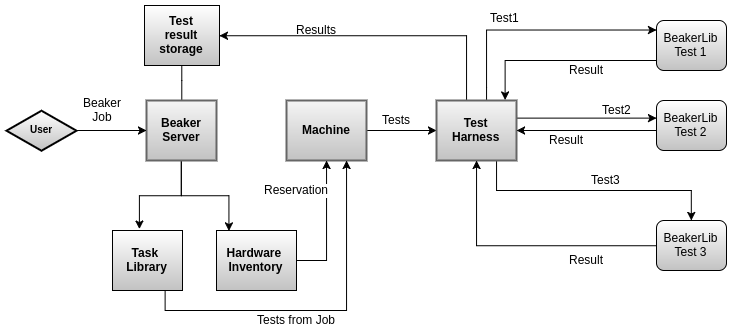
\includegraphics[width=\linewidth]{beaker_relations.png}
  \caption{Beaker relation to BeakerLib}
  \label{fig:beaker_relation}
\end{figure}

\chapter{BeakerLib}
\label{beakerlib_chapter}

This chapter takes a closer look on inner workings of BeakerLib, with focus on Journal feature and performance issues it suffers from. 

\section{Important functions}
As stated earlier BeakerLib is shell-level library with functions that make writing and running tests easier as well as examining their results.
BeakerLib adds testing functions to \texttt{shell} functionality, so user can combine normal \texttt{shell} commands and constructions with helping functions which can make writing tests and examining their results easier. There is close to 80 of these functions (also known as \textbf{rlCommands}), description of most used ones follows:
\begin{itemize}
\item \texttt{rlRun()} - First argument of this function is any \texttt{shell} command, which is executed by \texttt{rlRun()}. Second is an expected \texttt{exit code} of first argument, it can contain one or more codes. Third argument is a comment. BeakerLib logs \texttt{FAIL} or \texttt{PASS} if expected exit code differs or not from actual one respectively along with comment. This is most used and important function.
\item \texttt{rlPass()} - Manual assertion and logging of \texttt{PASS}. Useful when in combination with if statement which user doesn't want to appear in logs but still wants to log its result. Reciprocal function \texttt{rlFail()} exists as well.
\item \texttt{rlAssertExists} - Asserts whether file given as a first argument exists.
\item \texttt{rlAssertGrep()} - Function logs \texttt{PASS} when pattern given as first argument matches in a file which is given a second argument. Optional flags are passed to \texttt{grep} and behave the same way.
\item \texttt{rlAssertRpm()} - Function asserts \texttt{PASS} when package given as first argument is installed.  Optional arguments allow specifying particular version, release or arch of the package.
\item \texttt{rlAssertDiffer()} - Asserts whether two files given as argument differ in their content. 
\item \texttt{rlJournalStart()} - This function is used at the start of each test. It is essential for proper run of the test as it initializes BeakerLib's  outputs, which described later in this chapter. Reciprocal function \texttt{rlJournalEnd()} must be called at the end of the test.
\item \texttt{rlPhaseStart()} - This function starts user-defined phase. Function takes two arguments, first one is a type of phase, second one is a name. Phase must be ended by calling \texttt{rlPhaseEnd()}. Phases are more closely explained in the next section.
\end{itemize}

\section{Phases}
BeakerLib divides tests into logical groups called Phases. There are three predefined types of phases:
\begin{itemize}
\item Setup - Preparing conditions for the test (such as creating temporary files, starting needed system services and so on), started by calling \texttt{rlPhaseStartSetup()}.
\item Test - Main phase for testing, started by calling \texttt{rlPhaseStartTest()}.
\item Cleanup - Reverting changes made by the test, started by calling \mbox{\texttt{rlPhaseStartCleanup()}}.
\end{itemize}

Apart from predefined Phases, user can also define own phases by calling \texttt{rlPhaseStart()} function. First argument of the function is a one of two types phase can have:

\begin{itemize}
\item WARN - if any rlCommand in phase of this type fails, whole phase will result in Warning state.
\item FAIL - similar to previous type however this time resulting in Failed state.
\end{itemize}

Basic phases Setup and Cleanup are WARN type, Test phase is a FAIL type.

The result of the whole test is the same as the worst result of any phase in the order: Failed, Warning, Passed.
Asserts must not be used outside of phases, if such a case occurs, a new phase opened, its result set to FAIL, then adding the stray assert into the new phase and finally to end it. 

This division helps with examining the result of test as it shows which phase, if any, causes fail in BeakerLib's output. 
example test \ref{lst:test_example} shows how basic BeakerLib test looks.

\begin{minipage}{\linewidth}
\begin{lstlisting}[style=beakerlib_bash,caption={BeakerLib basic test example},label={lst:test_example}]
# Include Beaker environment
. /usr/bin/rhts-environment.sh || exit 1
. /usr/share/beakerlib/beakerlib.sh || exit 1

PACKAGE=beakerlib
# Start of Journal
rlJournalStart
    # Start of Setup Phase, creating temp directory where test will take place 
    rlPhaseStartSetup
        rlAssertRpm $PACKAGE
        rlRun "TmpDir=\$(mktemp -d)" 0 "Creating tmp directory"
        rlRun "pushd $TmpDir"
    rlPhaseEnd
   # Start of Test Phase, testing touch and ls commands
    rlPhaseStartTest
        rlRun "touch foo" 0 "Creating the foo test file"
        rlAssertExists "foo"
        rlRun "ls -l foo" 0 "Listing the foo test file"
    rlPhaseEnd
   # Statr of Cleanup phase, temp directory is deleted
    rlPhaseStartCleanup
        rlRun "popd"
        rlRun "rm -r $TmpDir" 0 "Removing tmp directory"
    rlPhaseEnd
rlJournalPrint
rlJournalEnd
\end{lstlisting}
\end{minipage}

\section{BeakerLib's output}
BeakerLib produces three kinds of outputs. Two file formats and a console one in case of local testing or three file formats when testing remotely.

\subsection{journal.txt}
\textit{journal.txt} is a plain text file with human readable record of test's progress. After end of each phase, copy of the file is sent to Beaker for storage. Snippet of \textit{journal.txt} generated by Example test \ref{lst:test_example} is shown in \ref{lst:journaltxt_example}.

\begin{minipage}{\linewidth}
\begin{lstlisting}[style=txt,caption={Example of journal.txt},label={lst:journaltxt_example}]
::::::::::::::::::::::::::::::::::::::::::::::::::::::::::::::::::::::::::::::::
:: [   LOG    ] :: Setup
::::::::::::::::::::::::::::::::::::::::::::::::::::::::::::::::::::::::::::::::
:: [   PASS   ] :: Checking for the presence of beakerlib rpm 
:: [   LOG    ] :: Package versions:
:: [   LOG    ] ::   beakerlib-1.15-1.fc25.noarch
:: [   PASS   ] :: Creating tmp directory (Expected 0, got 0)
:: [   PASS   ] :: Command 'pushd /tmp/tmp.3iXfiT4GiR' (Expected 0, got 0)
:: [   LOG    ] :: Duration: 1s
:: [   LOG    ] :: Assertions: 3 good, 0 bad
:: [   PASS   ] :: RESULT: Setup
::::::::::::::::::::::::::::::::::::::::::::::::::::::::::::::::::::::::::::::::
:: [   LOG    ] :: Test
::::::::::::::::::::::::::::::::::::::::::::::::::::::::::::::::::::::::::::::::
:: [   PASS   ] :: Creating the foo test file (Expected 0, got 0)
:: [   PASS   ] :: File foo should exist 
:: [   PASS   ] :: Listing the foo test file (Expected 0, got 0)
:: [   LOG    ] :: Duration: 0s
:: [   LOG    ] :: Assertions: 3 good, 0 bad
:: [   PASS   ] :: RESULT: Test
::::::::::::::::::::::::::::::::::::::::::::::::::::::::::::::::::::::::::::::::
:: [   LOG    ] :: Cleanup
::::::::::::::::::::::::::::::::::::::::::::::::::::::::::::::::::::::::::::::::
:: [   PASS   ] :: Command 'popd' (Expected 0, got 0)
:: [   PASS   ] :: Removing tmp directory (Expected 0, got 0)
:: [   LOG    ] :: Duration: 0s
:: [   LOG    ] :: Assertions: 2 good, 0 bad
:: [   PASS   ] :: RESULT: Cleanup
::::::::::::::::::::::::::::::::::::::::::::::::::::::::::::::::::::::::::::::::
:: [   LOG    ] :: /performance/beakerlib/Performance/example_test
::::::::::::::::::::::::::::::::::::::::::::::::::::::::::::::::::::::::::::::::
:: [   LOG    ] :: Phases: 3 good, 0 bad
:: [   PASS   ] :: RESULT: /performance/beakerlib/Performance/example_test

\end{lstlisting}
\end{minipage}

\subsection{Console output}
\label{console_out}
If the executed test is connected to an \texttt{interactive shell} similar, human-readable, output to the \textit{journal.txt} is also printed to console's standard output (\texttt{stdout}). Apart from  \textit{journal.txt}'s content console's output is complemented by executed command's output. Also \texttt{shell}'s output is colored for increased readability.  Figure \ref{fig:console_output} shows snippet of such output.

\begin{figure}
  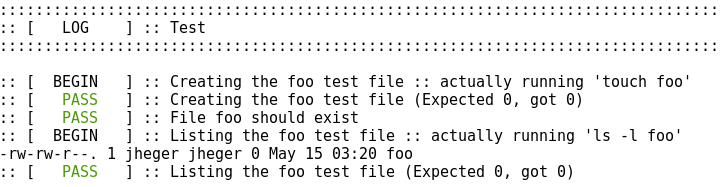
\includegraphics[width=\linewidth]{console_output.png}
  \caption{Snippet from console's output}
  \label{fig:console_output}
\end{figure}

\subsection{TESTOUT.log}
If the executed test is not connected to an \texttt{interactive shell}, the same text generated for Console's output is printed into the file \textit{TESTOUT.log}. This is mostly the case when executing a test remotely (in Beaker for example), where it is not possible to see the Console output.

\subsection{journal.xml}
Last output is a an XML\footnote{eXtensible Markup Language} file. XML is a markup language, designed to store and transport data\cite{xml_intro}.

\textit{journal.xml} is stripped off of executed commands' own output, but core information (such as which commands were executed, whether they passed or failed and so on) is kept. Also metadata about the test run (time of execution, which component was tested and more) as well as information about the hardware and software test was run on are added. \textit{journal.xml} is sent back to Beaker same as \textit{journal.txt} where it is available for further processing by automated tools. It also serves as a source of information about current state of the test during its execution, for example whether there is currently an open phase or how many failed tests or phases there are so far. Example of \textit{journal.xml} generated by Example test \ref{lst:test_example} is shown in \ref{lst:journalxml_example}.

\begin{minipage}{\linewidth}
\begin{lstlisting}[style=xml_journal,caption={Example of journal.xml},label={lst:journalxml_example}]
<?xml version="1.0"?>
<BEAKER_TEST>
  <package>beakerlib</package>
  <pkgdetails sourcerpm="beakerlib-1.15-1.fc25.src.rpm">
beakerlib-1.15-1.fc25.noarch </pkgdetails>
  <beakerlib_rpm>beakerlib-1.15-1.fc25</beakerlib_rpm>
  <beakerlib_redhat_rpm>beakerlib-redhat-1-6.fc16</beakerlib_redhat_rpm>
  <starttime>2017-05-15 09:47:44 CEST</starttime>
  <endtime>2017-05-15 09:47:45 CEST</endtime>
  <testname>/performance/beakerlib/Performance/example_test</testname>
  <release>Fedora release 25 (Twenty Five)</release>
  <hostname>localhost.localdomain</hostname>
  <arch>x86_64</arch>
  <hw_cpu>4 x Intel(R) Core(TM) i7-6600U CPU @ 2.60GHz</hw_cpu>
  <hw_ram>19496 MB</hw_ram>
  <hw_hdd>459.8 GB</hw_hdd>
  <purpose>PURPOSE of /performance/beakerlib/Performance/example_test
Description: example test created by beaker-wizard
Author: Jakub Heger &lt;jheger@redhat.com&gt;
</purpose>
  <log>
    <phase endtime="2017-05-15 09:47:45 CEST" name="Setup" result="PASS" 
score="0" starttime="2017-05-15 09:47:44 CEST" type="WARN">
      <pkgdetails sourcerpm="beakerlib-1.15-1.fc25.src.rpm">
beakerlib-1.15-1.fc25.noarch </pkgdetails>
      <test message="Checking for the presence of beakerlib rpm ">PASS</test>
      <message severity="LOG">Package versions:</message>
      <message severity="LOG">  beakerlib-1.15-1.fc25.noarch</message>
      <test command="TmpDir=$(mktemp -d)" message="Creating tmp directory (Expected 0, got 0)">
PASS</test>
      <test command="pushd /tmp/tmp.3iXfiT4GiR" 
message="Command 'pushd /tmp/tmp.3iXfiT4GiR' (Expected 0, got 0)">PASS</test>
    </phase>
    <phase endtime="2017-05-15 09:47:45 CEST" name="Test" result="PASS" score="0" 
starttime="2017-05-15 09:47:45 CEST" type="FAIL">
      <pkgdetails sourcerpm="beakerlib-1.15-1.fc25.src.rpm">
beakerlib-1.15-1.fc25.noarch </pkgdetails>
      <test command="touch foo" message="Creating the foo test file (Expected 0, got 0)">PASS</test>
      <test message="File foo should exist ">PASS</test>
      <test command="ls -l foo" message="Listing the foo test file (Expected 0, got 0)">PASS</test>
    </phase>
    <phase endtime="201-05-16 09:47:45 CEST" name="Cleanup" result="PASS" score="0" 
starttime="2017-05-15 09:47:45 CEST" type="WARN">
      <pkgdetails sourcerpm="beakerlib-1.15-1.fc25.src.rpm">
beakerlib-1.15-1.fc25.noarch </pkgdetails>
      <test command="popd" message="Command 'popd' (Expected 0, got 0)">PASS</test>
      <test command="rm -r /tmp/tmp.3iXfiT4GiR" 
message="Removing tmp directory (Expected 0, got 0)">PASS</test>
    </phase>
    <message severity="LOG">JOURNAL XML: /var/tmp/beakerlib-dI2ochw/journal.xml</message>
    <message severity="LOG">JOURNAL TXT: /var/tmp/beakerlib-dI2ochw/journal.txt</message>
  </log>
</BEAKER_TEST>

\end{lstlisting}
\end{minipage}

\subsection{BeakerLib directory}
\label{beakerlib_dir}
Described files are saved into a BeakerLib test directory created for each individual test. 

If the test is run locally, temporary directory is created on system with \texttt{mktemp} command, which creates pseudo-random name.

If run on Beaker a unique \textbf{TESTID} is generated for each test. This ID serves as a name for test directory as well as an identifier which Beaker later uses when connecting test results with correct test. It is also important in case where restart is a regular part of a test. Upon restarting the test machine the same TESTIDs are relayed from Beaker to Harness with information which tests were already run. Harness then continues with execution of unfinished tests, starting with test that caused the restart, in the same BeakerLib directory it did before, where there are partial results of the test, so it can continue where it left off.

\section{Source files}
This section describes a few of BeakerLib's source files, relevant to this thesis.
\begin{itemize}
\item \textit{beakerlib.sh} - Starting point of every tests. It is \texttt{sourced} at the beginning of each test and in turn \texttt{sources} all other BeakerLib files.
\item \textit{testing.sh} - Contains definitions of the most used rlCommands as well as some internal functions.
\item \textit{journal.sh} - Provides Bash-side Journaling functionality. Functions from this file process information about what to log and relay them to \textit{journalling.py} (with \texttt{rlj} prefix) or query the \textit{journal.xml} to obtain information about the current state of the test(with standard \texttt{rl} prefix).
\item \textit{journalling.py} - \texttt{Python} script responsible for creating most of BeakerLib's outputs. It creates and modifies \textit{journal.xml} file.
\item \textit{logging.sh} - Complements \textit{journalling.py} in creating Console output by printing output produced but commands called with \texttt{lRun()}.
\end{itemize}

\section{Analysis of slow performance}
It was reported that BeakerLib suffers performance problems when running long tests. Time of processing each rlCommand grew longer after many (several hundreds and more) were used. Analysis of library was problematic due to lack of documentation, complex structure and uncommented code, however thorough investigation of the source code indicated that problem lies with generating \textit{journal.xml}. 

Script \textit{journalling.py} is called after each rlCommand to log its result into \textit{journal.xml}. This isn't big problem with small test as the \textit{journal.xml} file takes up only a few kilobytes, however when the file takes up dozens or hundreds of kilobytes, repeated loading the file from disk, parsing, adding a line of log and then saving the file back to the disk adds significantly more load to CPU\footnote{Central Processing Unit}. Running larger tests therefore becomes quite time consuming and considerably slows down testing as a whole.
This has been determined as the main focus of the thesis since it probably is the most significant performance bottleneck. Influence of used Harness was thought  to be negligible and won't be focused on in this thesis.

Figure \ref{fig:rl_run} illustrates simplified version of how \texttt{rlRun()} propagates through different functions from BeakerLib files (which are \texttt{sourced} at the time test execution,  depicted by rounded rectangles) and how it is logged into the Journal. Figure also partially reveals complicated environment of BeakerLib, where every rlCommand is processed by many internal functions, making understanding and developing BeakerLib problematic. 

\begin{figure}[h!]
  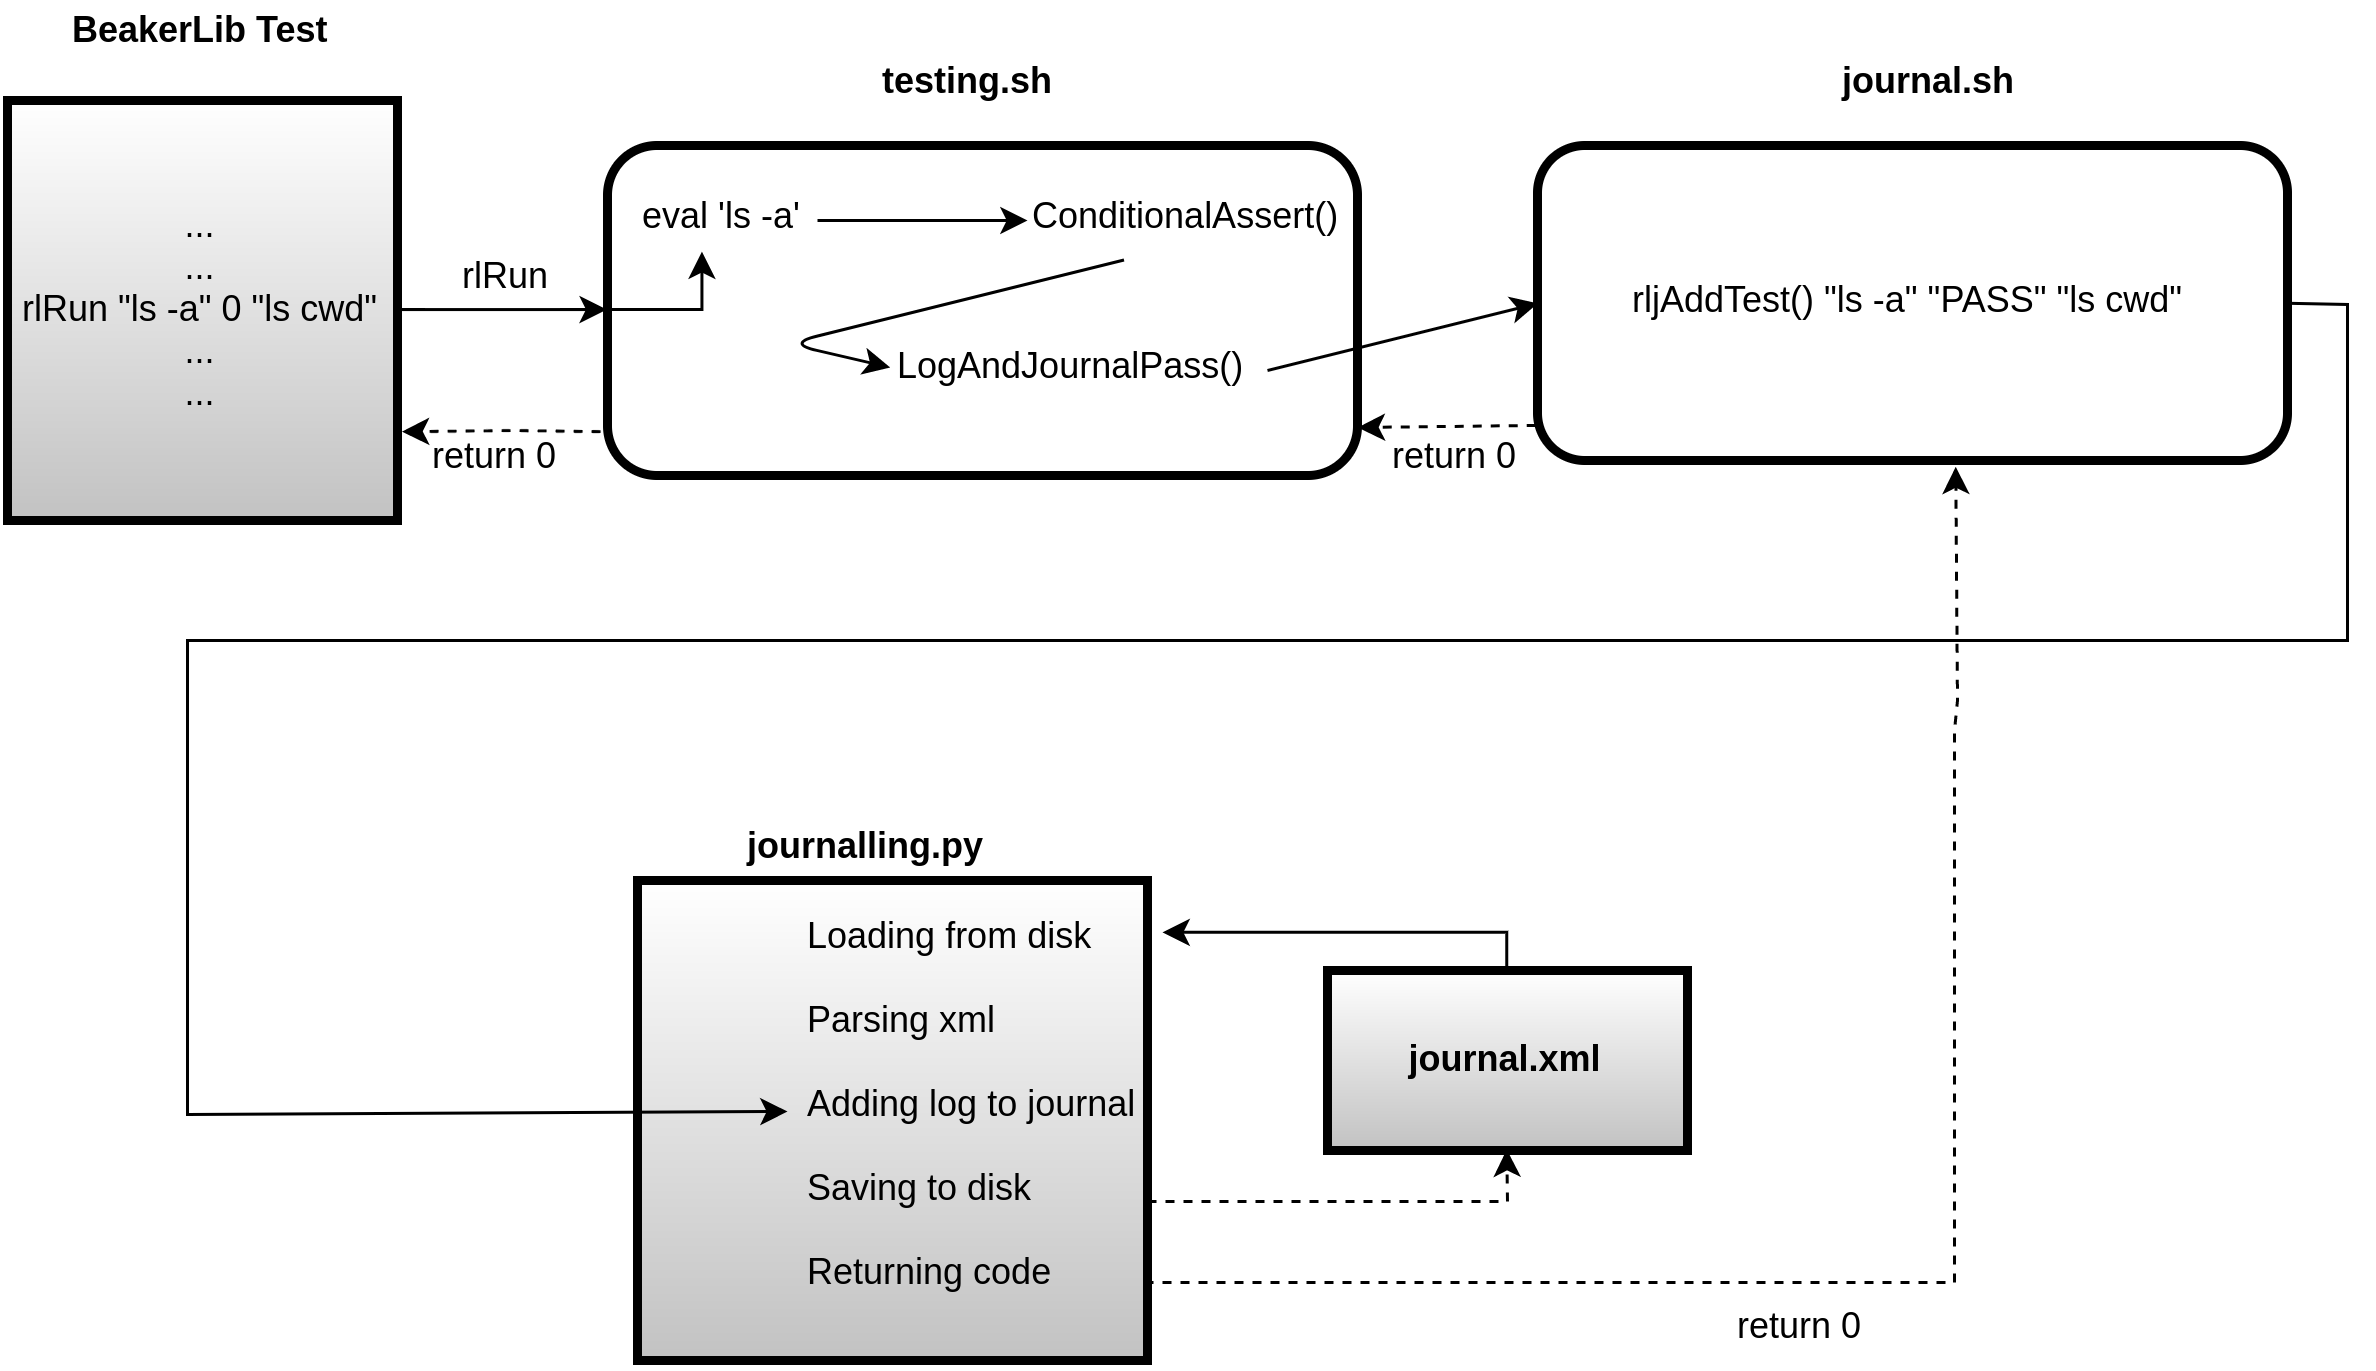
\includegraphics[width=\linewidth]{rl_run.png}
  \caption{Logging of rlRun to Journal}
  \label{fig:rl_run}
\end{figure}


The next chapter describes proposed solutions to analyzed problem with their pros and cons.


\chapter{Solution of Journaling problem}
\label{solutions}

Sections in this chapter provide possible solutions to the Journaling problem. Besides explaining the principle of each solution, the sections also discuss their advantages, disadvantages and potential issues.

\section{Change of xml parser}
XML parser is a program which can turn XML document into structured object in RAM\footnote{Random Access Memory}. Depending on implementation of the parser, that object is then easier to access by the program as it may provide methods to navigate the object and search it or potentially modify. 

Parsing of XML in BeakerLib is done by \textit{journalling.py} script by \texttt{Python} module \texttt{xml.dom.minidom}\cite{minidom_doc}. 

 \texttt{xml.dom.minidom} is a native part of \texttt{Python} from version 2.0 and provides minimal implementation of the DOM\footnote{Document Object Model} interface, with an API\footnote{Application Programming Interface} similar to that in other languages. 

I decided to change parser to different one, to measure whether it will provide better performance. Because of reasons of backward compatibility with RHEL 5\footnote{Red Hat Enterprise Linux 5} which needs to be supported by BeakerLib, the choice of XML parsers was limited to native modules of \texttt{Python 2.4.3}. Two additional XML parsers were present for given version.

\begin{itemize}
\item lxml - The \texttt{lxml} XML toolkit is a pythonic binding for the C libraries libxml2 and libxslt. It combines the speed and XML feature completeness of these libraries with the simplicity of a native \texttt{Python} API\cite{lxml_doc}.

It works similarly to \texttt{xml.dom.minidom} in the way that when reading XML object from a file, it will read it whole, builds an object out of it and provides methods for the object to allow access to it.
\item xml.sax  \cite{sax_doc} - \texttt{xml.sax} originated as a parser for \texttt{Java}\cite{Sax2}. In \texttt{Python} it was released with version 2.0. It differs from \texttt{xml.dom.minidom} and \texttt{lxml} where the two mentioned parsers work with a whole XML file,  \texttt{xml.sax} emits events as it goes step by step through the file\cite{sax_example}. Using this approach means less memory has to be allocated for XML handling and therefore makes it ideal when working with very large amount of XML  data.
\end{itemize}

I decided to implement \texttt{lxml} parser as it is supposed to be faster and less demanding on memory than \texttt{xml.dom.minidom}\cite{lxml_performance}, while keeping its intuitive interface.

\section{Change in calling journalling.py}
Next proposition to make BeakerLib faster is in a way \textit{journalling.py} is called. The assumption being that repeated parsing of XML document slows BeakerLib the most, reducing the number of times it was parsed was then the highest priority. 

\subsection{Queue file solution}  % ??? mbox
First solution is to create a new, temporary \textbf{queue file}, which will act as a kind of buffer. \mbox{rlCommands} will behave as before apart from creating BeakerLib journals, but instead they will write message into the queue file. This file will be read and processed only when necessary, that is at the end each phase, when journals are sent to Beaker.

\subsubsection{Disadvantages}
The way BeakerLib is designed now it in most cases expects some form of return value from \textit{journalling.py} immediately after adding a log to a journal. Performed logging either returns code indicating success of failure or \texttt{string} with information about the current state of test. This presents problem as there is no way how to communicate back these information when parsing is postponed. 

\subsection{Daemon-like solution}
Second solution is to rewrite \textit{journalling.py} script to have daemon-like behavior. 

\texttt{Daemons} in Unix are long-running background processes that answers requests for services\cite{daemon_explanation}.

This solution will run XML parser as a separate background process for each test. The XML object will be stored in memory, and parsed as whole only at the beginning of journal creation and in case of restarting the test run.  

This way BeakerLib can receive response about current test state immediately while still keeping CPU load minimal. Daemon-like solution however brings different obstacles.

\subsubsection{Disadvantages}
An independent, potentially long running process daemon is more vulnerable to unplanned events such as unexpected exit. This must be addressed by both daemon (to exit as safely as possible)  and by the rest of BeakerLib (to detect that daemon is no longer running and to behave accordingly). 

\subsubsection{Communication}
Inter-process communication between running test and daemon has to be created for test to inform which rlCommand is supposed to be logged and for daemon to respond with current state of XML document. This two-way communication must be synchronous to assure BeakerLib and daemon process their respective messages in correct order. I considered following options:

\begin{itemize}
\item Unix sockets  -  <expand>
\item Named pipes - Named pipes are device files. They allow inter-process communication by reading it and writing into is as if regular file, however under normal circumstances the read/write is a blocking operation\cite{pipes_blocking}. This means if one process opens pipe for reading, it will hang there until another process opens the pipe for writing. This feature can be used for synchronization of communication between processes. 
\end{itemize}

% DOPLINT CITACE ^^ ???

I chose to implement communication through Named pipes because synchronization issue is taken care of because of the way Named pipes are designed.


\chapter{Implementation of proposed solutions}
\label{implementations}
This chapter describes how the proposed solutions were implemented. Each solution has its own section that describes implementation details and obstacles that were found and had to be solved during the implementation.
During changing of parsers I discovered and fixed few bugs present in current implementation of \textit{journalling.py}.

\section{Change of XML parser}
\subsection{Differences in parsers}
As mentioned before I chose to change original XML parser to \texttt{lxml}. Only changes in source code were in file \textit{journalling.py} as it is only part of BeakerLib that directly works with journal's XML object. 
Most of the changes were in \texttt{xml.dom.minidom}'s method for creating new XML element and assigning value into it.
The biggest difference between given parsers is that \texttt{lxml} does not provide as many helping methods as \texttt{xml.dom.minidom} does.
For example in \texttt{lxml}  there is no method \texttt{getElementsByTagName()} to search XML object by a tag name. Instead \texttt{lxml} supports \texttt{xpath}\cite{xpath} syntax for searching the object. xpath\footnote{XML Path Language} is part of XSLT\footnote{eXtensible Stylesheet Language Transformations} standard. It be can used to navigate through elements and attributes in an XML document.

Another example of difference is an approach for accessing element's children. While \texttt{xml.dom.minidom} has dedicated methods and attributes such as \texttt{hasChildNodes()} which returns \texttt{bool} value or \texttt{childNodes} which is a iterable attribute of element's children, \texttt{lxml} has more low level implementation. It treats elements as \texttt{Python lists} so \texttt{hasChildNodes()} can be replaced with simple \texttt{len(element) != 0}.
\\
\\
Because preliminary performance measurement showed faster test execution with \texttt{lxml}, I decided to implement the rest of the proposed solutions with this parser.

\section{Queue file solution}
This section deals with implementation of queue file solution. It is divided into subsections that discuss files I designed or changed during implementation. 

\subsection{Queue file}
Queue file was designed in a way so it was simple to implement, in a human readable format for potential test debugging and easy to extend by new, future functions that will work with it. 
It is a plain text file, each line containing one buffered message for \texttt{Python} script to process later, on demand. Messages are kept in the same format as original solution uses for calling \textit{journalling.py} to preserve consistency with the exception that they are now escaped, which is described in section.

\subsection{journal.sh}
Creation of  queue file, by using \texttt{touch} command, was added to function \texttt{rlJournalStart()} which initializes Journaling functionality. Using \texttt{touch} assures that if the queue file already exists (which happens when test run is interrupted and started again), its content is not deleted (in case of restart of the testing machine as described in section \ref{beakerlib_dir}).

It now also \texttt{exports} new variable \texttt{BEAKERLIB\_QUEUE}, with queue file's path, into test's environment so \texttt{Python} script \textit{queued\_journalling.py}, can later access it.

Original calling of \textit{journalling.py} script, which is a main functionality of \textit{journal.sh}, was replaced in one of two ways:

\begin{itemize}
\item Delayed calling - New function \texttt{rljPrintToQueue()} takes all arguments that were originally meant for \textit{journalling.py} and instead prints them into the queue file, where it will be processed by \textit{queued\_journalling.py} later during execution of the test. This concerns functions which do not necessarily require response about current test state from \textit{journal.xml}.  In original solution responses to these functions were only \texttt{exit codes} which they did not utilize in any way or if they did theirs functionality was re-implemented. Namely functions that use delayed calling are: \texttt{rlJournalPrint()}, \texttt{rljAddTest()}, \texttt{rljAddMetric()}, \texttt{rljAddMessage()}, \texttt{rljRpmLog()}
\item Immediate calling of \textit{queued\_journalling.py} - Essentially the same as the original solution. These functions require immediate response. Using this way of calling won't save on any CPU load (in fact the the load will be slightly higher than before because of operations related to queue file processing), however in typical BeakerLib test these functions are in minority compared to previous type of calling.  Functions and the response they require are:  
\begin{itemize}
\item \texttt{rlJournalStart()} - requires confirmation that journal was initiated successfully
\item \texttt{rlJournalPrintText()} - requires \textit{journal.txt} which is generated from current \mbox{\textit{journal.xml}}
\item \texttt{rlGetTestState()}  - requires number of failed asserts in the test so far
\item \texttt{rlGetPhaseState()} - requires number of failed phases in the test so far
\item \texttt{rljAddPhase()} - requires immediate print of name of the new phase to Console output
\item \texttt{rljClosePhase()} - requires result of closed phase, to send it to Beaker along with Journal
\item \texttt{rlJournalEnd()} - requires immediate print of \textit{journal.txt} which is generated from \textit{journal.xml}
\end{itemize}
\end{itemize}

Function \texttt{rljAddTest()} is the cause of the most calls of \textit{journalling.py} in original solution, therefore had the highest need to be moved into group of functions with Delayed calling. However it does require knowledge of current state of the test. That being situation when Assert (rlCommand using \texttt{rljAddTest()} for Journaling) is used outside of a phase, such information is held only in current \textit{journal.xml}. To solve this problem functionality of  \texttt{rljAddTest()} had to moved into \textit{queued\_journalling.py} script, discussed in the next subsection.

Apart from printing to queue file, \texttt{rljPrintToQueue()} also has to escape given arguments. This needs to be d
one because firstly some of the arguments originating from user may contain newline character which would break the"one buffered command per line" rule in  queue file's format and secondly so \textit{queued\_journalling.py} may process it with \texttt{optparse} module.
Escaping is done with \texttt{printf} Bash builtin\cite{bash_builtins}, specifically its \texttt{\%q} option which causes \texttt{printf} to output in \texttt{shell-quoted} format.

\subsection{queued\_journalling.py}
File \textit{queued\_journalling.py} originated from \textit{journalling.py} but it differs in several ways.

Now when it is called, it first parses current \textit{journal.xml} and then calls new method \texttt{updateXML()} with parsed XML object as an argument. This method opens queue file and finds last line it accessed in previous call. From there it reads buffered lines, parses each with \texttt{Python}'s \texttt{optparse} module and modifies the XML object accordingly in the similar way it did originally, this time however without parsing \textit{journal.xml} each time as the XML object is passed as an argument to appropriate methods. 

When it reaches end of file, it makes a mark (by adding a line at the end of the queue file with a number already processed lines) for future readings and returns to the original call coming from one of the \textit{journal.sh}'s  Immediate calling functions. After modification from that function it generates response and returns it to \textit{journal.sh}. 

Exceptions to this behavior are:
\begin{itemize}
\item \texttt{rlJournalStart()} - This function doesn't access queue file but only initializes XML object and returns an \texttt{exit code} whose value depends on whether the initialization was successful 
\item \texttt{rlJournalEnd()} - This one makes sure every buffered command was processed as it is an exit point from the test and so last opportunity to modify \textit{journal.xml}
\end{itemize}

As mentioned in previous subsection, functionality of  \texttt{rljAddTest()} had to be altered. Given that Bash side of BeakerLib had no way of knowing if the test was added outside of phase at the time of writing this operation into the queue file, this action had to be resolved when \textit{queued\_journalling.py} processed the queue file. 
New method \texttt{testOutOfPhase()} was implemented which is called when assertion outside of phase is detected and it performs the same process as when this event happened in original \textit{journal.sh}, described in chapter \ref{beakerlib_chapter} in section Phases.

\subsection{Problems with implementation}
Main goal of this solution was to reduce number of times \textit{journal.xml} is parsed, by delaying as many Journaling operations as possible, while keeping BeakerLib's outputs the same. The way BeakerLib is designed now it is not possible, because some information is always lost when operations are delayed. In case of this implementation I was able to keep \textit{journal.xml}, and therefore \textit{journal.txt}  as well, the same as with original solution, however at the price Console's output (therefore \textit{TESOUT.log}'s too as it is Console's output printed to file) which is now missing all information usually given by functions from Delayed calling category. Only complementary output created by functions from \textit{logging.sh} remain.

Solving this issue would require more extensive changes to BeakerLib's design which I decided not to implement for now so Queue file solution remains only as a proof of concept.

\section{Daemon-like solution}
This section describes individual changes I made to BeakerLib's design in order to implement Daemon-like solution.

\subsection{journal.sh}
Function \texttt{rlJournalStart()} in this implementation creates Named pipe using \texttt{mkfifo} and then \texttt{exports} its path into environment.
Then it spawns \textit{daemon\_journalling.py} process in the background with \texttt{\&} operator and stores its \texttt{PID\footnote{Process identifier}}.

Every call of \textit{journalling.py} in original implementation was replaced with new function \texttt{rljCallDaemon()}, which takes the same arguments as original function. When this new function is called it firstly escapes given arguments using similar way as in queue file, this time however another function had to be created.  \texttt{rljCallDaemon()} passes its argument to the function \texttt{escapeArguments()} which uses \texttt{printf} and \texttt{echo} Bash builtins to escape arguments in loop which are then caught back in \texttt{rljCallDaemon()} with \texttt{\$()} construct\cite{command_substitution} for catching output. It is implemented this way to avoid using temporary file.

After arguments are escaped, \texttt{rljCallDaemon()} checks whether the daemon is still running with \texttt{kill -0 \$DAEMON\_PID} call. 

\texttt{kill} program is used to send signals to processes. If used with \texttt{-0} option, no signal is actually sent but error checking against the process is still performed and it returns \texttt{0} when process with given PID is running\cite{man_kill}. This is done to make sure the daemon is still running before pipe writing operation.  If the daemon wasn't running before writing to pipe, the test would hang there indefinitely, so if the daemon is not running, the test exits with error.

After this check is performed, \texttt{rljCallDaemon()} writes to Named pipe escaped message, where it waits until daemon reads it and responds. Response is read as a next action, decoded from a format that will be discussed in the next subsection and then the response is returned to function that called \texttt{rljCallDaemon()}. 
This is repeated until end of the test is reached, where function \texttt{rljJournalEnd()} sends \texttt{signal} with \texttt{kill} to end the daemon.



Function \texttt{rlJournalPrintText()} had to be reworked slightly. This function generates \textit{journal.txt} output from \textit{journal.xml} and has two main usages:
\begin{itemize}
\item It is a standard part of BeakerLib test where it is called directly right before test ends by calling \texttt{rlJournalEnd()}. It prints  \textit{journal.txt} to \texttt{stdout} if the test is connected to \texttt{interactive shell}.
\item It is used by internal functions during test execution to continuously generate partial \textit{journal.txt} files and send them back to Beaker if using Beaker and harness or storing them to disk when no harness is used.
\end{itemize}

Reworked function now accepts one optional argument and passes it to \texttt{rljCallDaemon()} and it was added to all currently implemented BeakerLib functions that call \texttt{rlJournalPrintText()}. In original solution there was a simple way how to have \textit{journalling.py} print either to \texttt{stdout} or to catch the same output into variable using  \texttt{\$()} construct or redirecting it to a file, because each call of  \textit{journalling.py} was a separate process whose output could be controlled. When using daemon however, this is no longer possible, either all output would be caught or none at all.
A way how to differentiate which \textit{journalling.py}'s output is supposed to be printed to \texttt{stdout} and which is supposed to be returned to \textit{journal.sh} through Named pipe had to be implemented. Functions that need to catch the daemon's output now use  \texttt{rlJournalPrintText()} with the optional argument. How it affects \textit{daemon\_journalling.py} is described in next subsection.
Currently unused function \texttt{rlJournalPrint()} was reworked is the same way.

\subsection{journalling\_daemon.py}
\textit{journalling.py} script again originates from \textit{journalling.py}. This time however, it is designed to run in endless loop, instead of returning after one executed action.

Before the daemon enters the endless loop, it performs checks whether environment is prepared for it (whether Named pipe exists or it can access test's PID). Only if all checks are successfully verified it enters the loop, otherwise exits with error. 

In each iteration it checks whether test's  process is still running analogously to how \texttt{rljCallDaemon()} does it. Then it reads the Named pipe and waits there until \texttt{rljCallDaemon()} writes to it. After message is read, method \texttt{parseAndProcess()} is called and it parses the message and acts upon it. 

If the message received comes from \texttt{rlJournalStart()} the XML object is initialized and stored in \texttt{global} variable \texttt{jrml} so it its accessible to all other methods that use the XML object.

As was stated in previous subsection, change in outputting behavior had to be implemented. When optional argument \texttt{toVar} is detected all functions related to printing instead of \texttt{print} function store their respective outputs in variables. These are gradually appended to each other and at the end of all printing they are instead returned through Named pipe back to \textit{journal.sh} where individual functions can catch them.

Any other message call the same methods as in original implementation with the difference which is that now the methods use the \texttt{global jrnl}.

When a message is processed, \texttt{parseAndProcess()} must encode the response, because original implementation was able to respond with either \texttt{return code} or \texttt{string} and this solution is only ably to respond with \texttt{string}. Simple format \texttt{message:X-code:Y}, where X is replace with \texttt{string} and Y with \texttt{return code}, was implemented which is quickly decoded by \texttt{rljCallDaemon()} using Regular expression\cite{regex}.

\subsection{Signals}
Signals are asynchronous interrupts that are used for inter-process communication. Signals are usually used by the operating system to notify processes that some event occurred\cite{signals}. For example when operating system plans to reboot, it sends signal to all running processes to inform them that reboot will take place. \texttt{rlJournalEnd()} in daemon-like solution sends signal \texttt{SIGTERM} to end \textit{daemon\_journalling.py}'s process where it is caught and handled by daemon's \texttt{signal handler}.

Signal handlers are functions that are called when program receives signal to handle the event properly. In daemon solution Signal handlers were added to both daemon and Bash side of BeakerLib.

In \textit{daemon\_journalling.py} method \texttt{signalHandler()} was created. It it set to handle most common signals, that would cause it to exit improperly. When such signal is received, daemon interrupts what is currently doing and through \texttt{signalHandler()} calls \texttt{saveAndExit())} method which saves current state of XML object to disk and exits.

\textit{journal.sh} uses \texttt{trap} command to catch signals. Upon receiving signal it \texttt{kills} daemon to always make sure that daemon will not stay running in the background after test is unexpectedly ended.  

\subsection{Problems with implementation}
Using background processes with blocking operations is a rather volatile solution. In a case of some unanticipated event it may happen one side or the other may be hung up on blocking operation with no process to unblock it, even though Signal handlers were implemented to lower the chance of such a situation to happen.

During testing of this solution such behavior was not reproduced. However testing on much larger scale, including different operating systems, CPU architectures and other testing conditions, would have be concluded to confirm it is unlikely such event could occur. 


\section{Verification of implemented solutions}
Verification that implemented optimizations didn't cause regression, was directed on \textit{journal.xml} as it is a main focus point of this thesis. Due to its nature automated verification was problematic to implement, because two \textit{journal.xml} files generated from one test may differ in many ways while both still being valid (they may differentiate in such information as time of execution, hardware/software specifications or even in reported results, as test could pass or fail independently on BeakerLib implementation).

Because of this reasons only manual verification took place.

\chapter{Performance testing}
\label{performance}

This chapter explains what performance testing is and why is ti done. Then it describes what tests and in which environments were used to measure performance of BeakerLib before and after optimizations were implemented.


Performance testing is a type of \textbf{non-functional testing}, that is testing whose goal is to test quality characteristics of a component, rather than its functionality\cite{non-functional_testing}.

For performance testing of BeakerLib I chose two kinds of tests in in two kinds of testing environments. They are described in following sections.

\section{Tests}

\subsection{Artificial tests}
First type of tests are artificial tests created by me with \texttt{beaker-wizard} tool to specifically target and measure performance of Journaling modifications I made. They consist mostly of rlCommands that directly work with \textit{journalling.py} (ot its variants of implemented modifications), for example commands \texttt{rlLog()} or \texttt{rlPhaseStart()} and \texttt{rlPhaseEnd()}. This way we can observe clear difference in performance without being affected by operations unrelated to Journaling (executing actions that verify functionality of components in real tests). 

\begin{itemize}
\item Test1 - Test used as and example \ref{lst:test_example}. It is a very short test and for which proposed solutions were not aimed therefore increase in performance with this test is not expected. Test contains 17 rlCommands.
\item Test2 - Test contains 1000 calls of function \texttt{rlLog()} divided into 3 phases. This function requires very little overhead and so its results represent direct performance difference caused by implementations however they do not represent performance difference when running typical BeakerLib test. Test contains 1014 rlCommands.
\item Test3 - Test consists of 500 calls functions of \texttt{rlPhaseStartTest()} and \texttt{rlPhaseEnd()}. Even thought it has the same length as Test2, this test is expected to run longer because phase controlling rlCommands have larger overhead when working with \textit{journal.xml}. Test contains 1014 rlCommands.
\item Test4 - Test comprises of 500 phases with a few typical rlComands inside them. This test resembles typical BeakerLib the most out of all artificial ones and is longest as well. Test contains 3013 rlCommands.
\end{itemize}

These tests are included in Appendix \ref{appendix:cd} in directory tests/.

\subsection{Real tests}
Second type are real tests used in Red Hat. These are examples of tests that have been reported to have bad performance with BeakerLib so I am testing them to see if my modifications have real life impact on its performance. 

Finding such tests was problematic because real tests are often written specifically for particular hardware or software and behave differently under different circumstances. The challenge then was not only to find long running tests but most importantly tests that all have the same behavior on one specific remote machine as well as on my local machine used for testing.

\begin{itemize}
\item Test1
\item Test2
\end{itemize}

\section{Testing Environment}

\subsection{Local}
First environment is local laptop for convenience and speed of execution. Tests were run directly, without any harness and with these technical specifications:  %??? psudoharness

\begin{center}
    \begin{tabular}{| l | l |}
    \hline
    Model & Lenovo T460s \\ \hline
    CPU & 4 cores Intel(R) i7-6600U, 2.60GHz \\ \hline
    CPU architecture & x86\_64 \\ \hline
    RAM & 19496 MB   \\ \hline
    Operating System & Fedora release 25 \\ \hline
    \end{tabular}
\end{center}

\subsection{Remote in beaker}
Second round of testing was done to emulate real testing conditions and to verify that changes made to BeakerLib do not break functionality outside of controlled environment. Tests were run u the default test harness Beah. Technical specification were following:

\begin{center}
    \begin{tabular}{| l | l |}
    \hline
    CPU & 1 core Intel(R) Xeon, 2.10GHz \\ \hline
    CPU architecture & x86\_64 \\ \hline
    RAM & 2847 MB   \\ \hline
    Operating System & Red Hat Enterprise Linux Server 7.3 \\ \hline
    \end{tabular}
\end{center}


\section{Measured Values} % ??? value
Goal of this thesis was to optimize performance in regards to time of execution, so that is only the value that was measured. Values were obtained from \textit{journal.xml} which has builtin mechanisms to track how long took the execution of the test.

\section{Baseline measurements}
This section shows measured time of execution in seconds of each test with the original implementation. Each test was run 15 times and results were then averaged. Complete data set is located in Appendix \ref{appendix:data}.

\shorthandoff{-}
\begin{center}
    \begin{tabular}{| c | c | c |}
    \hline
    \multirow{2}{*}{\textbf{Test}} & \textbf{Local} & \textbf{Remote} \\ \cline{2-3}
    & \textbf{Average time} & \textbf{Average Time} \\ \hline
    Test 1 & 20 & 20 \\ \hline
    Test 2 & 25 & 20  \\ \hline
    Test 3 & 20 & 20 \\ \hline
    Test 4 & 89 & 20 \\ \hline
    Test 5 & 20 & 20 \\ \hline
    Test 6 & 20 & 20 \\ \hline
    Test 7 & 20 & 20 \\ \hline
    Test 8 & 20 & 20 \\ \hline
    \end{tabular}
\end{center}
\shorthandon{-}

\section{Implemented optimizations}
This presents measured time of execution in seconds of each test with each of the implemented optimizations. Each test was run 15 times and results were then averaged. Complete can be seen in Appendix \ref{appendix:data}.

\subsection{lxml parser}

\shorthandoff{-}
\begin{center}
    \begin{tabular}{| c | c | c |}
    \hline
    \multirow{2}{*}{\textbf{Test}} & \textbf{Local} & \textbf{Remote} \\ \cline{2-3}
    & \textbf{Average time} & \textbf{Average Time} \\ \hline
    Test 1 & 20 & 20 \\ \hline
    Test 2 & 25 & 20  \\ \hline
    Test 3 & 20 & 20 \\ \hline
    Test 4 & 89 & 20 \\ \hline
    Test 5 & 20 & 20 \\ \hline
    Test 6 & 20 & 20 \\ \hline
    Test 7 & 20 & 20 \\ \hline
    Test 8 & 20 & 20 \\ \hline
    \end{tabular}
\end{center}
\shorthandon{-}

\subsection{Queue file solution with lxml parser}

\shorthandoff{-}
\begin{center}
    \begin{tabular}{| c | c | c |}
    \hline
    \multirow{2}{*}{\textbf{Test}} & \textbf{Local} & \textbf{Remote} \\ \cline{2-3}
    & \textbf{Average time} & \textbf{Average Time} \\ \hline
    Test 1 & 20 & 20 \\ \hline
    Test 2 & 25 & 20  \\ \hline
    Test 3 & 20 & 20 \\ \hline
    Test 4 & 89 & 20 \\ \hline
    Test 5 & 20 & 20 \\ \hline
    Test 6 & 20 & 20 \\ \hline
    Test 7 & 20 & 20 \\ \hline
    Test 8 & 20 & 20 \\ \hline
    \end{tabular}
\end{center}
\shorthandon{-}

\subsection{Daemon solution with lxml parser}

\shorthandoff{-}
\begin{center}
    \begin{tabular}{| c | c | c |}
    \hline
    \multirow{2}{*}{\textbf{Test}} & \textbf{Local} & \textbf{Remote} \\ \cline{2-3}
    & \textbf{Average time} & \textbf{Average Time} \\ \hline
    Test 1 & 20 & 20 \\ \hline
    Test 2 & 25 & 20  \\ \hline
    Test 3 & 20 & 20 \\ \hline
    Test 4 & 89 & 20 \\ \hline
    Test 5 & 20 & 20 \\ \hline
    Test 6 & 20 & 20 \\ \hline
    Test 7 & 20 & 20 \\ \hline
    Test 8 & 20 & 20 \\ \hline
    \end{tabular}
\end{center}
\shorthandon{-}


\chapter{Analysis of results}
\label{results}

\chapter{Conclusion}
\label{conclusion}
Recap of results
\\
Future work


%=========================================================================
